\documentclass[journal,12pt,twocolumn]{IEEEtran}

\usepackage{setspace}
\usepackage{gensymb}

\singlespacing


\usepackage[cmex10]{amsmath}

\usepackage{amsthm}

\usepackage{mathrsfs}
\usepackage{txfonts}
\usepackage{stfloats}
\usepackage{bm}
\usepackage{cite}
\usepackage{cases}
\usepackage{subfig}

\usepackage{longtable}
\usepackage{multirow}

\usepackage{enumitem}
\usepackage{mathtools}
\usepackage{steinmetz}
\usepackage{tikz}
\usepackage{circuitikz}
\usepackage{verbatim}
\usepackage{tfrupee}
\usepackage[breaklinks=true]{hyperref}
\usepackage{graphicx}
\usepackage{tkz-euclide}
\usepackage{float}

\usetikzlibrary{calc,math}
\usepackage{listings}
    \usepackage{color}                                            %%
    \usepackage{array}                                            %%
    \usepackage{longtable}                                        %%
    \usepackage{calc}                                             %%
    \usepackage{multirow}                                         %%
    \usepackage{hhline}                                           %%
    \usepackage{ifthen}                                           %%
    \usepackage{lscape}     
\usepackage{multicol}
\usepackage{chngcntr}

\DeclareMathOperator*{\Res}{Res}

\renewcommand\thesection{\arabic{section}}
\renewcommand\thesubsection{\thesection.\arabic{subsection}}
\renewcommand\thesubsubsection{\thesubsection.\arabic{subsubsection}}

\renewcommand\thesectiondis{\arabic{section}}
\renewcommand\thesubsectiondis{\thesectiondis.\arabic{subsection}}
\renewcommand\thesubsubsectiondis{\thesubsectiondis.\arabic{subsubsection}}


\hyphenation{op-tical net-works semi-conduc-tor}
\def\inputGnumericTable{}                                 %%

\lstset{
%language=C,
frame=single, 
breaklines=true,
columns=fullflexible
}
\begin{document}
\newtheorem{theorem}{Theorem}[section]
\newtheorem{problem}{Problem}
\newtheorem{proposition}{Proposition}[section]
\newtheorem{lemma}{Lemma}[section]
\newtheorem{corollary}[theorem]{Corollary}
\newtheorem{example}{Example}[section]
\newtheorem{definition}[problem]{Definition}

\newcommand{\BEQA}{\begin{eqnarray}}
\newcommand{\EEQA}{\end{eqnarray}}
\newcommand{\define}{\stackrel{\triangle}{=}}
\bibliographystyle{IEEEtran}
\providecommand{\mbf}{\mathbf}
\providecommand{\pr}[1]{\ensuremath{\Pr\left(#1\right)}}
\providecommand{\qfunc}[1]{\ensuremath{Q\left(#1\right)}}
\providecommand{\sbrak}[1]{\ensuremath{{}\left[#1\right]}}
\providecommand{\lsbrak}[1]{\ensuremath{{}\left[#1\right.}}
\providecommand{\rsbrak}[1]{\ensuremath{{}\left.#1\right]}}
\providecommand{\brak}[1]{\ensuremath{\left(#1\right)}}
\providecommand{\lbrak}[1]{\ensuremath{\left(#1\right.}}
\providecommand{\rbrak}[1]{\ensuremath{\left.#1\right)}}
\providecommand{\cbrak}[1]{\ensuremath{\left\{#1\right\}}}
\providecommand{\lcbrak}[1]{\ensuremath{\left\{#1\right.}}
\providecommand{\rcbrak}[1]{\ensuremath{\left.#1\right\}}}
\theoremstyle{remark}
\newtheorem{rem}{Remark}
\newcommand{\sgn}{\mathop{\mathrm{sgn}}}
\providecommand{\abs}[1]{\vert#1\vert}
\providecommand{\res}[1]{\Res\displaylimits_{#1}} 
\providecommand{\norm}[1]{\lVert#1\rVert}
%\providecommand{\norm}[1]{\lVert#1\rVert}
\providecommand{\mtx}[1]{\mathbf{#1}}
\providecommand{\mean}[1]{E[ #1 ]}
\providecommand{\fourier}{\overset{\mathcal{F}}{ \rightleftharpoons}}
%\providecommand{\hilbert}{\overset{\mathcal{H}}{ \rightleftharpoons}}
\providecommand{\system}{\overset{\mathcal{H}}{ \longleftrightarrow}}
	%\newcommand{\solution}[2]{\textbf{Solution:}{#1}}
\newcommand{\solution}{\noindent \textbf{Solution: }}
\newcommand{\cosec}{\,\text{cosec}\,}
\providecommand{\dec}[2]{\ensuremath{\overset{#1}{\underset{#2}{\gtrless}}}}
\newcommand{\myvec}[1]{\ensuremath{\begin{pmatrix}#1\end{pmatrix}}}
\newcommand{\mydet}[1]{\ensuremath{\begin{vmatrix}#1\end{vmatrix}}}
\numberwithin{equation}{subsection}
\makeatletter
\@addtoreset{figure}{problem}
\makeatother
\let\StandardTheFigure\thefigure
\let\vec\mathbf
\renewcommand{\thefigure}{\theproblem}
\def\putbox#1#2#3{\makebox[0in][l]{\makebox[#1][l]{}\raisebox{\baselineskip}[0in][0in]{\raisebox{#2}[0in][0in]{#3}}}}
     \def\rightbox#1{\makebox[0in][r]{#1}}
     \def\centbox#1{\makebox[0in]{#1}}
     \def\topbox#1{\raisebox{-\baselineskip}[0in][0in]{#1}}
     \def\midbox#1{\raisebox{-0.5\baselineskip}[0in][0in]{#1}}
\vspace{3cm}
\title{ASSIGNMENT 4}
\author{Ananthoju Pranav Sai \\ AI20BTECH11004}
\maketitle
\newpage
\bigskip
\renewcommand{\thefigure}{\theenumi}
\renewcommand{\thetable}{\theenumi}
Download all python codes from 
\begin{lstlisting}
https://github.com/Ananthoju-Pranav-Sai/EE3900/blob/main/Assignment-4/codes/Assignment-4.py
\end{lstlisting}
%
and latex-tikz codes from 
%
\begin{lstlisting}
https://github.com/Ananthoju-Pranav-Sai/EE3900/tree/main/Assignment-4/Assignment-4.tex
\end{lstlisting}
%
\section{Linear Forms 2.37}
Find the coordinates of the point where the line through $\myvec{5\\1\\6}$ and $\myvec{3\\4\\1}$ crosses the ZX-plane.
%
\section{Solution}
The equation of line joining A and B is given by 
\begin{align}
    \vec{r} &= \vec{A}+\lambda(\vec{B}-\vec{A})   
\end{align}
General equation of plane is given by
\begin{align}
    \vec{n}^T\vec{r} = c
\end{align}
where $\vec{n}$ is normal vector to the plane 
\begin{align}
    \vec{n} = \myvec{n_1\\n_2\\n_3}
\end{align}
\begin{lemma}
    The point of intersection of line
    \begin{align}
        \vec{r} &= \vec{A}+\lambda(\vec{B}-\vec{A})
    \end{align}
    and plane
    \begin{align}
        \vec{n}^T\vec{r} = c  
    \end{align}
    is given by
    \begin{align}
        \vec{r_0} = \vec{A}+\brak{\frac{c-\vec{n}^T\vec{A}}{\vec{n}^T(\vec{B}-\vec{A})}}(\vec{B}-\vec{A})
    \end{align}
\end{lemma}
\begin{proof}
Let $r_0$ be the point of intersection of the line and the plane then the point lies on both line and plane so,
\begin{align}
    \vec{r_0} &= \vec{A}+\lambda(\vec{B}-\vec{A})  
\end{align}
As $r_0$ also lies on plane
\begin{align}
    &\vec{n}^T\vec{r_0} = c\\
    \implies &\vec{n}^T(\vec{A}+\lambda(\vec{B}-\vec{A})) = c\\
    \implies &\lambda\vec{n}^T(\vec{B}-\vec{A}) = c-\vec{n}^T\vec{A}\\
    \implies &\lambda = \brak{\frac{c-\vec{n}^T\vec{A}}{\vec{n}^T(\vec{B}-\vec{A})}}
\end{align}
Therefore,
\begin{align}
    \vec{r_0} = \vec{A}+\brak{\frac{c-\vec{n}^T\vec{A}}{\vec{n}^T(\vec{B}-\vec{A})}}(\vec{B}-\vec{A})
\end{align}
\end{proof}
Given,
\begin{align}
    \vec{A} = \myvec{5\\1\\6}\\
    \vec{B} = \myvec{3\\4\\1}
\end{align}
Equation of line joining A and B is given by 
\begin{align}
    \vec{r} &= \vec{A}+\lambda(\vec{B}-\vec{A})\\
\end{align}
Equation of ZX-plane is given by
\begin{align}
    &y=0\\
    \implies &\vec{n}=\myvec{0\\1\\0}, c=0
\end{align}
Therefore coordinates of the intersection point are
\begin{align}
   \vec{r_0} = \vec{A}+\brak{\frac{c-\vec{n}^T\vec{A}}{\vec{n}^T(\vec{B}-\vec{A})}}(\vec{B}-\vec{A}) 
\end{align}
substituting all the vectors gives,
\begin{align}
    \vec{r_0} = \frac{1}{3}\myvec{17\\0\\23}
\end{align}
\begin{figure}[!ht]
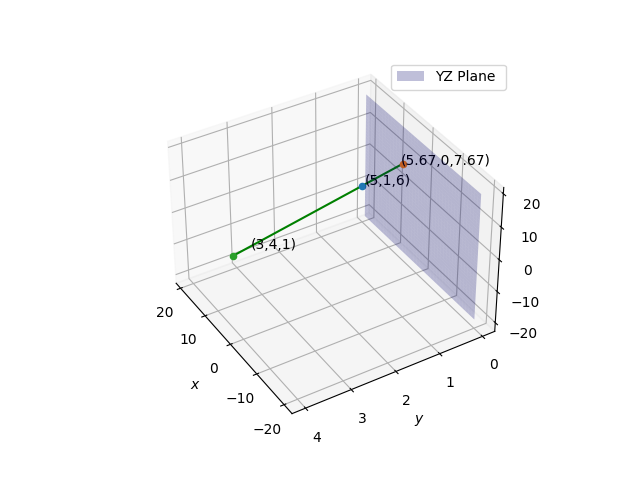
\includegraphics[ width=\columnwidth]{Line_AB.png}
\caption{Line and point of intersection}
\label{fig:Line }	
\end{figure}
\end{document}